\chapter{State of the Art}
\label{cap:state-of-the-art}

\section{Self-Adaptive Software Systems}
\label{sec:sas}
In modern-day applications, software complexity has extremely increased thanks to the spread of highly available and faster wireless connection such as in the Internet of Things (IoT) ambit. Since software is often deployed in dynamic contexts, where requirements, environment assumptions and usage profiles varies continuously, software complexity increased over time to the point where it is often composed by a number of sub-components and/or sub-services that work together in order to offer a service to the users. This is the case of service-oriented applications -- also called Service Based Systems (SBS) -- that are composed by multiple \emph{services} and \emph{components}. In these systems, services offered by third-party providers are dynamically composed into workflows to deliver complex functionalities, so SBSs rely on self adaptation to cope with the uncertainties associated with third-party services as the loose coupling of services makes a reconfiguration feasible. Without adaptation, the application is prone to degraded performance  because of faulty components, messages lost between services or delays due to an increasing number of users.

During the past decade a lot of research has been made in this scope but the engineering of adaptive systems remains a incredible challenge.\cite{soft-eng-for-sas-2} In order to solve the problem, \textbf{Self-Adapting Software Systems (SASS)} are born. These are flexible systems that can adapt themselves to their contextual needs and can do so with the highest performance and availability. General discussion concerning the issue and the state of the art in the design and implementation have been presented.\cite{soft-eng-for-sas-2}\cite{survey-aut-comp}\cite{self-adap-soft}\cite{soft-eng-for-sas-1}\cite{soft-eng-for-sas-3}\cite{arch-based-appr-to-sas}\cite{sas-quant-ver} 

These kind of systems have some fundamental properties called auto-managing that are:
\begin{itemize}
	\item Auto-configuration
	\item Auto-recovery in case of failure
	\item Auto-optimization
	\item Auto-protection
\end{itemize}
All these properties can be grouped in two more abstract concepts which are self-awareness and context-awareness.

\textbf{Self-Awareness} is the ability of the system to be able to monitor itself in terms of available resources and behavior.

\textbf{Context-Awareness} is the ability of the system to understand the environment where it is working, using the information provided by its components, and adapt itself to all the changes that can occur during its normal operational status.
To better understand how a SASS works we need to answer some simple questions:
\begin{itemize}
	\item Who is adapting?
	\item Which adaptation is required?
	\item When is necessary to adapt?
	\item Where is needed to change something?
	\item Why is needed an adaptation?
	\item How we achieve this goal?
\end{itemize}

During the past years have been developed some dimensions that help to answer all this simple questions: \emph{Time}, \emph{Reason}, \emph{Level}, \emph{Technique} and \emph{Adaptation Control} shown in figure \ref{fig:dimensions}.
\begin{figure}[h]
	\centerline
	{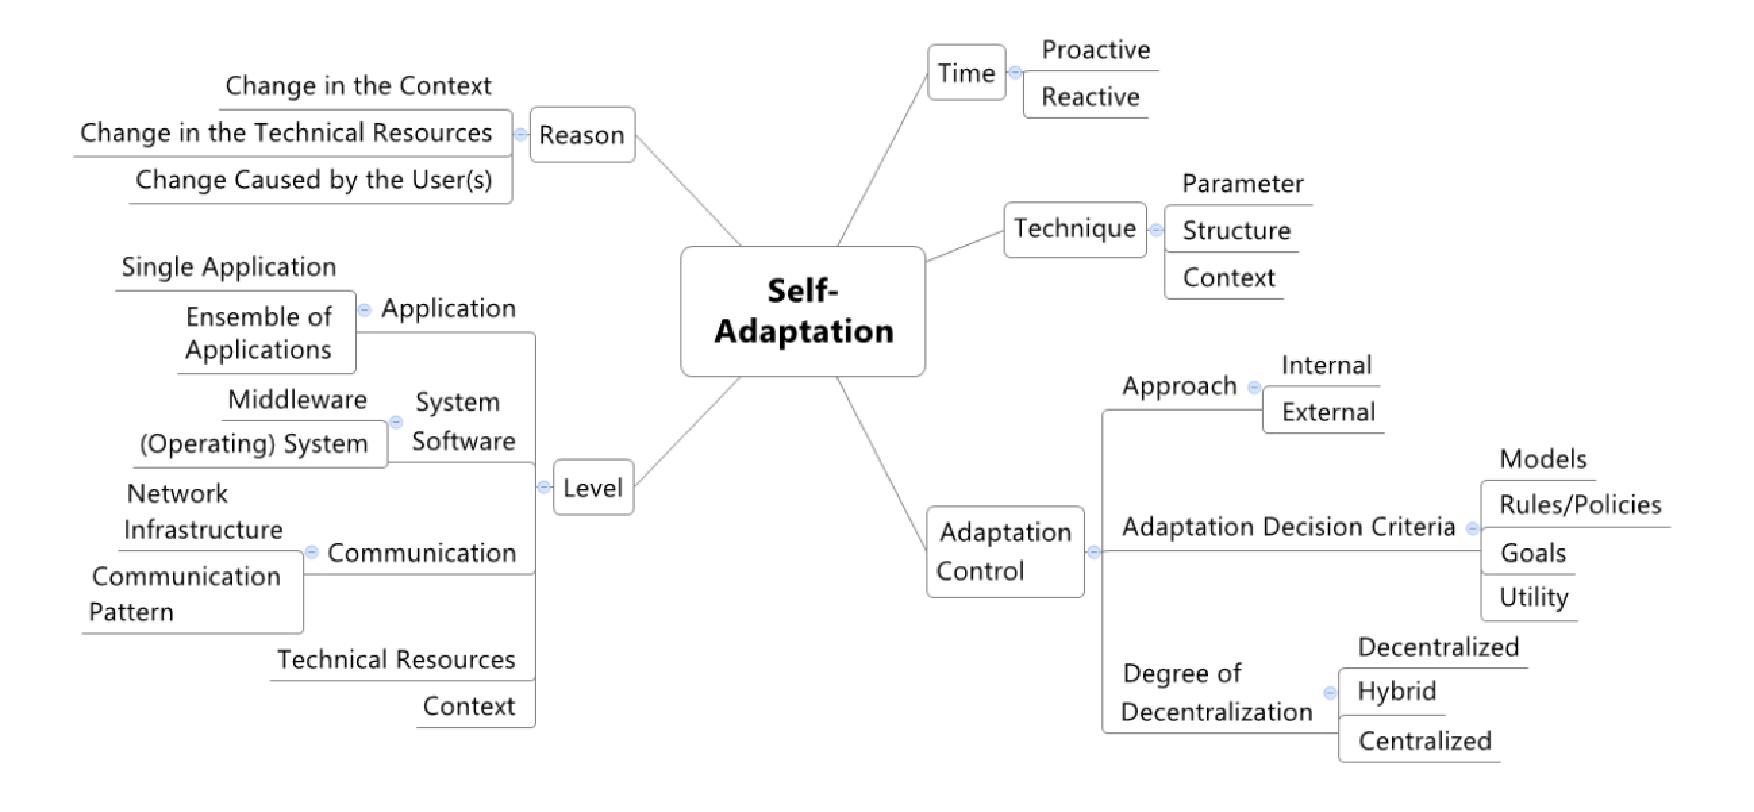
\includegraphics[scale=0.55]{img/dimensions.pdf}}
	\caption[The Dimensions]{The Dimensions to analyze adaptation.\cite{eng-appr-sas}}
	\label{fig:dimensions}
\end{figure}

\textbf{Who is adapting?} As the name suggests, it's the system itself that changes something in order to preserve some given constraint.

\textbf{Which adaptation is required?} The \emph{Technique} dimension is the one that answers this question in fact the software engineer can change either the parameters or the system can be considered as a set of components. The former case allows to fine tuning the system at the expense of an higher complexity, the latter is called composite vision and permits the systems to cooperate exchanging algorithms and much more important, reusing components which improve performance because failed or defected components can be replaced.

\textbf{When is necessary to adapt?} The \emph{Time} dimension is crucial in this situation. There are three typical approaches: the reactive one is the more traditional one which states that an adaptation is needed only after a causative event. The other two approaches are more interesting and they are predictive and proactive. The former studies the system before any event and calculate the need of an adaptation, the latter applies and adaptation despite an event and improves the performance. From the user perspective the proactive approach is the best because it doesn't interrupt the operation of the system in any load but it is the more complicated to implement. Monitoring continuously the system is a costly task to do, on the other side an adaptive monitoring is simple that analyze only specific aspect and/or resources and intervenes only if needed.

\textbf{Where is needed to change something?} In general a SASS is composed by two main part: the the adaptability logic (AL) and the managed resource (MR). The former in general doesn't change, the latter is composed at the base of the hardware and of the software such as the operating system or, in case of distributed systems, the middleware that control the hardware; at a higher level of the application. These are the parts that require adaptation. To answer this question is needed to decide at which level the operation has to be applied without neglecting the relationship between the MR and the AL which is composed by the network that connects them and/or the view of the communication patterns. Thus \emph{Level} is the considered dimension.

\textbf{Why is needed an adaptation?} In this case, \emph{Reason} is the right dimension. There can be one or more reason because a system needs adaptation such as a change in the available resources, a change in the environment or a change in the user base of the system.

\textbf{How we achieve this goal?} The answer to this question is more complicated than the others so is treated in the following section using the \emph{Adaptation Control}.

\subsection{Adaptation Control}


\section{The SOLAR Framework}
However working on the adaptability of a system can impact other quality attributes such as performance, reliability or maintainability and in the worst case improving adaptability can decrease part, if not all, of these attributes as stated in \cite{bass2003software}: \emph{quality attributes can never be achieved in isolation, the achievement of any one will have an effect, sometimes positive and sometimes negative, on the achievement of others}.

Find a balance between these quality attributes is often a challenging task because sometimes they're conflicting each other, e.g. lower cost and higher availability, so find an adaptability value that can meet all the requisites is, as a consequence, a challenging task too.




